%-----------------------------------------------
% Template para criação de resumos de projectos/dissertação
% jlopes AT fe.up.pt,   Fri Jul  3 11:08:59 2009
%-----------------------------------------------

\documentclass[9pt,a4paper]{extarticle}

%% English version: comment first, uncomment second
%\usepackage[portuguese]{babel}  % Portuguese
\usepackage[english]{babel}     % English
\usepackage{graphicx}           % images .png or .pdf w/ pdflatex OR .eps w/ latex
\usepackage{times}              % use Times type-1 fonts
\usepackage[utf8]{inputenc}     % 8 bits using UTF-8
\usepackage{url}                % URLs
\usepackage{multicol}           % twocolumn, etc
\usepackage{float}              % improve figures & tables floating
\usepackage[tableposition=top]{caption} % captions
\usepackage{mathtools}
%% English version: comment first (maybe)
\usepackage{indentfirst}        % portuguese standard for paragraphs
%\usepackage{parskip}

%% page layout
\usepackage[a4paper,margin=30mm,noheadfoot]{geometry}

%% space between columns
\columnsep 12mm

%% headers & footers
\pagestyle{empty}

%% figure & table caption
\captionsetup{figurename=Fig.,tablename=Tab.,labelsep=endash,font=bf,skip=.5\baselineskip}

%% heading
\makeatletter
\renewcommand*{\@seccntformat}[1]{%
  \csname the#1\endcsname.\quad
}
\makeatother

%% avoid widows and orphans
\clubpenalty=300
\widowpenalty=300


\begin{document}

\title{\vspace*{-8mm}\textbf{\textsc{Software Repository Mining Analytics to Estimate Software Component Reliability}}}
\author{\emph{André Freitas - freitas.andre@fe.up.pt}\\[2mm]
\small{Thesis supervised by \emph{Prof.\ Rui Maranhão and Alexandre Perez}}}
\date{}
\maketitle
%no page number
\thispagestyle{empty}

\vspace*{-4mm}\noindent\rule{\textwidth}{0.4pt}\vspace*{4mm}

\begin{multicols}{2}

\section{Motivation}\label{sec:motiva}
Software plays an important role in society and in our daily routines, since we
rely on Software to communicate, manage information, etc. Software development
is relatively complex and the cost of fixing bugs can be up to 90\% of project's
cost \cite{Servant1}.

Software repositories have hidden valuable information that can be explored with
Machine Learning and Analytics techniques, to support Software defect prediction
models.

Crowbar \footnote{\url{http://crowbar.io/}} is an automatic fault localization
tool, that after an execution of tests, estimates faulty components. The
Barinel algorithm, used in this tool, uses static estimations
\cite{Abreu:2009:SMF:1747491.1747511}. They can be replaced with dynamic estimations
from defect prediction, to improve the quality of diagnosis.

\section{Goals}\label{sec:goals}

The main goals are:

\begin{itemize}
\item Predict defects from the analysis of Software repositories, learning what
are the most important variables to analyze and create a defect prediction model
based from existing techniques;
\item Improve the quality of diagnosis of Crowbar with the results from defect
prediction.
\end{itemize}

\section{Work}\label{sec:work}
It was developed a tool in Python named Schwa, that is capable
of analysing Git repositories and estimate the probability of a certain component
be defective. For example, Schwa is able to estimate that a certain file has
a certain probability of having a defect. If the file is Java code, the granularity
is until the method, so this means that we can estimate the probability of classes
and methods being defective.

\subsection{Installation}
Schwa is available for free at Github and
\footnote{\url{https://github.com/andrefreitas/schwa}} and can be installed by:
\begin{verbatim}
    pip install schwa --pre
\end{verbatim}

\subsection{Usage of the tool}
Schwa can be invoked as a command line utility with the following syntax:

\begin{verbatim}
  schwa git/repo/path [--commits COMMITS]
\end{verbatim}

The number of commits is optional, so you can analyze only the last changes. The
graphical report is available in fig. \ref{fig:sunburst}.

\begin{figure}[H]
\centerline{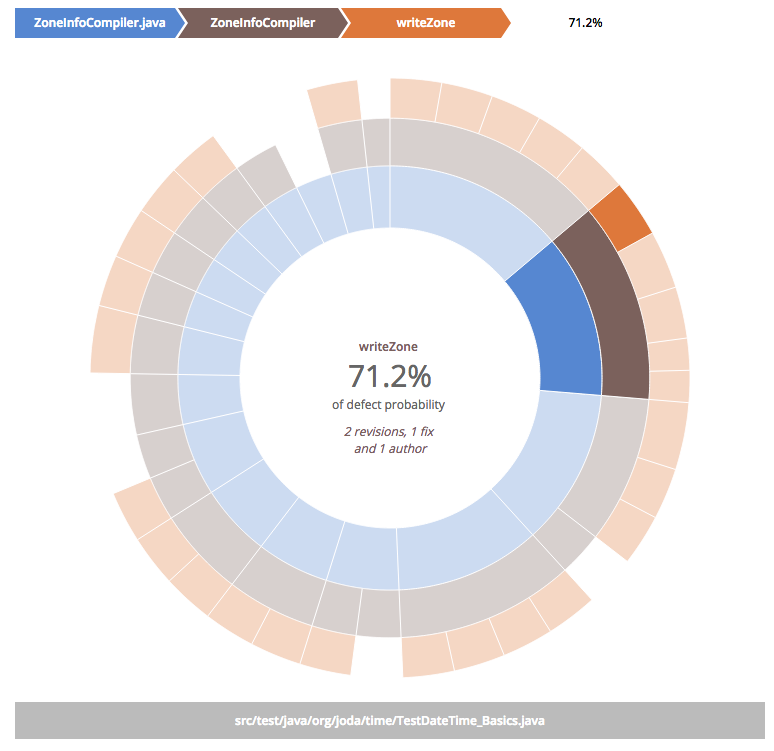
\includegraphics[scale=.25]{sunburst.png}}
\caption{Schwa report}
\label{fig:sunburst}
\end{figure}

In the graphic of fig. \ref{fig:sunburst} it is possible to inspect a hierarchy
of components(files, classes or methods). The center displays the estimation of
the defect probability along with the values of other collected metrics such as
revisions, fixes and authors of the component.

\subsection{Extraction}
The first phase of Schwa's process is the extraction of relevant data from the
repository for the analysis. By using GitPython
\footnote{\url{https://github.com/gitpython-developers/GitPython}} in each
commit we extract the message, author, timestamp and the list of changed components.

Parsing of Java code changes is possible by using the Plyj
\footnote{\url{https://github.com/musiKk/plyj}} library that was been
modified to include information from lines in classes and methods.

\subsection{Analysis}
The analysis phase uses the following principles:

\begin{itemize}
\item \textbf{Principle of revisions} Components with more revisions have higher
probability of being defective\cite{859533};

\item \textbf{Principle of fixes} Past defects are correlated with future
defects\cite{Zimmermann:2007:PDE:1268984.1269057};

\item \textbf{Principle of authors} Authors is a predective variable of future
defects\cite{Moser:2008:CAE:1368088.1368114,D'Ambros:2012:EDP:2318097.2318149}.
\end{itemize}

The variables used in the analysis are revisions, fixes and authors. They are
collected with the following algorithm:

\begin{verbatim}
For each commit in the repository
  twr = compute twr
  For each component in the commit
    component.revisions += twr
    IF commit is bug fix
        component.fixes += twr
    If is new author
        component.authors += twr
\end{verbatim}

Instead of using counters, we use the \emph{Time-Weighted-Risk} (TWR) function that
have its maximum value when a component was changed recently. This function
receives a normalized timestamp\cite{Chris2013}.

\begin{equation}
twr(t_i) = \frac{1}{1 + e^{-12t_i + 12 }}
\end{equation}

\subsection{Defect prediction model}
For each component the score is computed:
\begin{equation}
\begin{multlined}score = revisions * revisions_{weight} \\
+ fixes * fixes_{weight} \\
+ authors * authors_{weight} \\
\end{multlined}
\end{equation}

Then is normalized to an estimation of probability:

\begin{equation}
defect_{probability} = 1 - e^{-score}
\end{equation}

\subsection{Experiments}
We have developed a technique that learns the importante of variables (revisions,
fixes and authors) with genetic algorithms. After Schwa learned with academic,
Open Source and enterprise projects, we concluded that the importance of variables
is not the same for all the projects.

By using Schwa in Crowbar, we reduced the diagnostic time. In the Joda Time project
the time was reduced from 1 hour to less than a minute.

\section{Conclusions}\label{sec:conclui}
We created a technique capable of predicting defects of Software components, by
analyzing Git repositories and displaying results in a visual report.

Current code review techniques can benefit from the usage of Schwa, allowing
developer to focus their resources where defects are.

%%English version: comment first, uncomment second
%\bibliographystyle{unsrt-pt}  % numeric, unsorted refs
\bibliographystyle{unsrt}  % numeric, unsorted refs
\bibliography{refs}

\end{multicols}

\end{document}
